\section{Results}
\subsection{Example with MNIST 3s and 4s}
Only the observations depicting either a 3 or a 4 will be considered in this example. These digits are chosen due to their distinct shapes, hence ease of classification. Since the purpose is to make the algorithm find the differences between the two different digits, the spatial dimensions will not be decomposed. This means that a so-called partial Tucker-decomposition will be conducted, hence $\bs{B}$ and $\bs{C}$ will be identity matrices. Now experimentally setting the rank to 2, the decomposition of $N$ stacked 3s and 4s becomes:
\begin{equation}
    \tensor{X}^{N\times 28\times 28} \approx \tensor{G}^{2 \times 28 \times 28} \times_1 \bs{A}^{N\times 2} \qquad \Leftrightarrow \qquad \bs{X}_{(1)} \approx \bs{A}^{N\times 2} \ \bs{G}^{2 \times 28\cdot 28}_{(1)}
\end{equation}
Where $\bs{A}$ is the loading matrix in the dimension corresponding to different pictures. With the rank equal to 2, $\bs{A}$ holds 2 values per picture that should ideally be separating the two digits that is to be trained. \autoref{fig:decompExample3_4} shows how the decomposition of the first 100 training examples turns out. It seems the decomposition is able how to find the "general 3" and the "general 4", and then simply use the loadings of $\bs{A}$ to specify how much of each it an observation is. \autoref{fig:loadingAMatrix} shows a scatter-plot of the values of $\bs{A}$ colored to show the loadings corresponding to 3s and 4s respectively. There is some overlap between the two clusters, but it seems that they can be fairly distinguished. Using the means of the 3s, 4s and overall as loadings in the decomposition yields the approximated pictures shown in \autoref{fig:loadingsOfA}b-d.

\begin{figure}
    \centering
    \begin{subfigure}{0.45\linewidth}
        \centering
        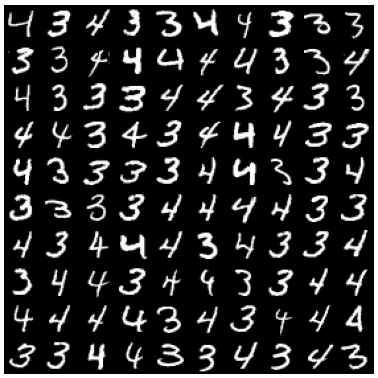
\includegraphics[width=\linewidth]{Pics/06_results/3_4_original.png}
        \captionsetup{width=.8\linewidth}
        \caption{Original MNIST training examples including only 3s and 4s.}
    \end{subfigure}
    \begin{subfigure}{0.45\linewidth}
        \centering
        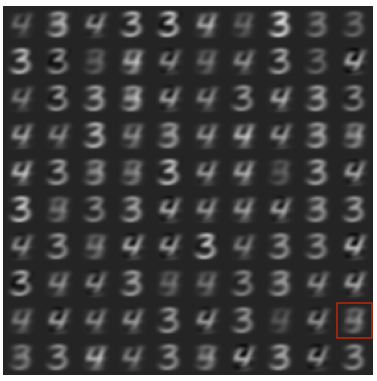
\includegraphics[width=\linewidth]{Pics/06_results/3_4_decomp.png}
        \captionsetup{width=.8\linewidth}
        \caption{Decomposed versions of the training examples on the left.}
    \end{subfigure}
    \captionsetup{width=.95\linewidth}
    \caption{MNIST training examples before and after decomposing with only rank 2 in the input dimension. Notice how the decomposed 3s and 4s look more standardized. It seems that every picture is a part standardized 3 and a part standardized 4. }
    \label{fig:decompExample3_4}
\end{figure}

\begin{figure}
    \centering
    \begin{subfigure}{0.99\linewidth}
        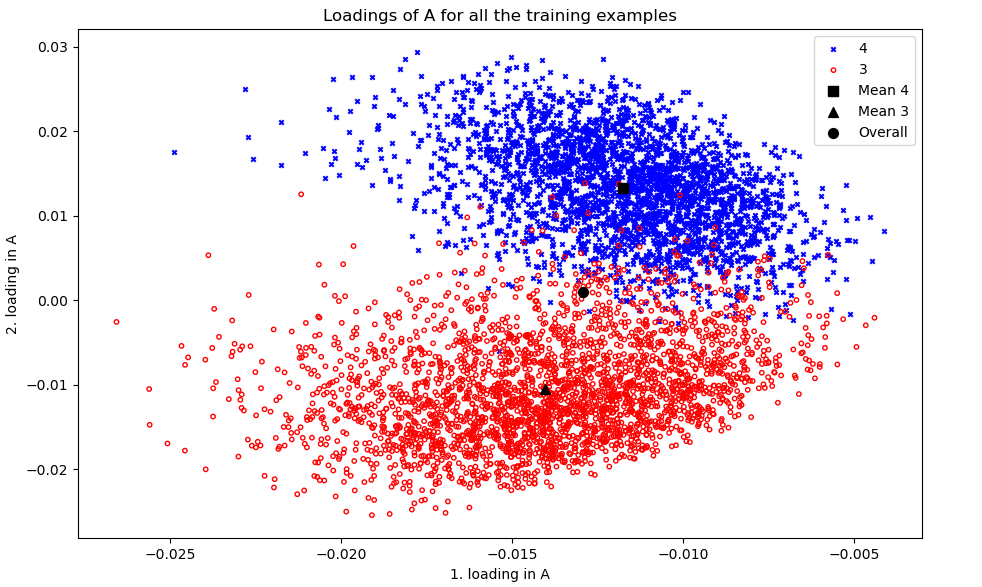
\includegraphics[width=\linewidth]{Pics/06_results/LoadingsOfAScatterMNIST.png}
        \caption{Scatter plot of the 2 loadings of the loading matrix $\bs{A}$ for the MNIST 3s and 4s respectively. The means of the 2 clusters and overall is also marked.}
        \label{fig:loadingAMatrix}
    \end{subfigure}
    \begin{subfigure}{0.3\linewidth}
    \centering
        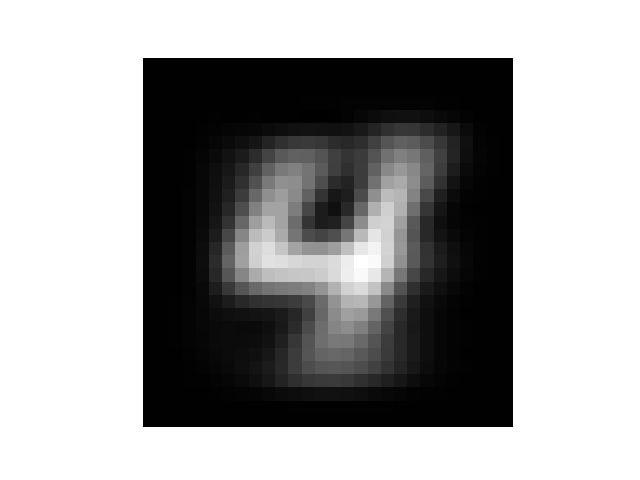
\includegraphics[width=.5\linewidth]{Pics/06_results/general4.png}
        \caption{The mean of 4s loadings}
    \end{subfigure}
    \begin{subfigure}{0.3\linewidth}
    \centering
        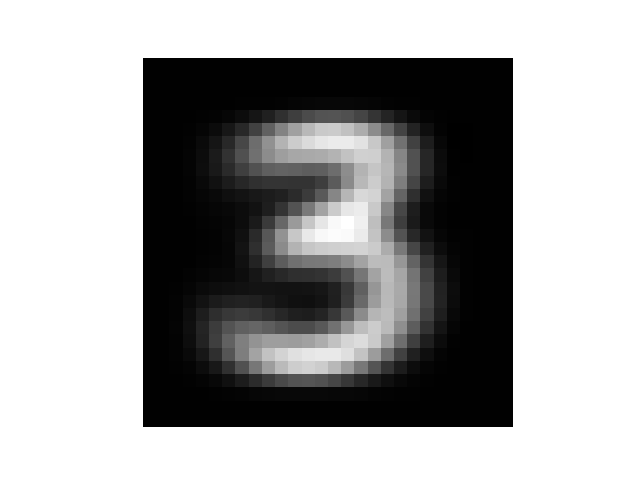
\includegraphics[width=.5\linewidth]{Pics/06_results/general3.png}
        \caption{The mean of 3s loadings}
    \end{subfigure}
    \begin{subfigure}{0.3\linewidth}
    \centering
        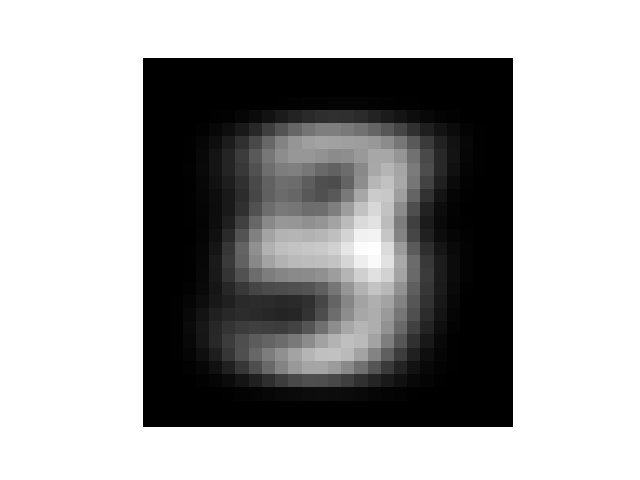
\includegraphics[width=.5\linewidth]{Pics/06_results/general.png}
        \caption{The mean of all loadings}
        \label{Hej}
    \end{subfigure}
    \caption{The 2 loadings of $\bs{A}$ for the MNIST 3s and 4s with means in the clusters and overall. Using the mean of the clusters as loadings in the decomposition gives the approximated "general" 3, 4 and overall given in \textbf{(b)-(d)}. Notice how the overall mean gives a mixture of a 3 and a 4. }
    \label{fig:loadingsOfA}
\end{figure}

This all comes down to the loadings of $\bs{A}$ holding a great deal of information about which pictures are 3s and which are 4s. This information could be used as input into the NN instead of the actual pictures potentially reducing the number of parameters dramatically (from 784 to 2 input neurons in this example). 